\chapter{Titolo del secondo capitolo}

\section{Introduzione}

Secondo capitolo della tesi. Esempio di citazione doppia \cite{Munoz-Lipo,Vas}.

Esempio di figura in fig.~\ref{FIG:Esempio di Figura}.

\begin{figure}[htbp]
\centering
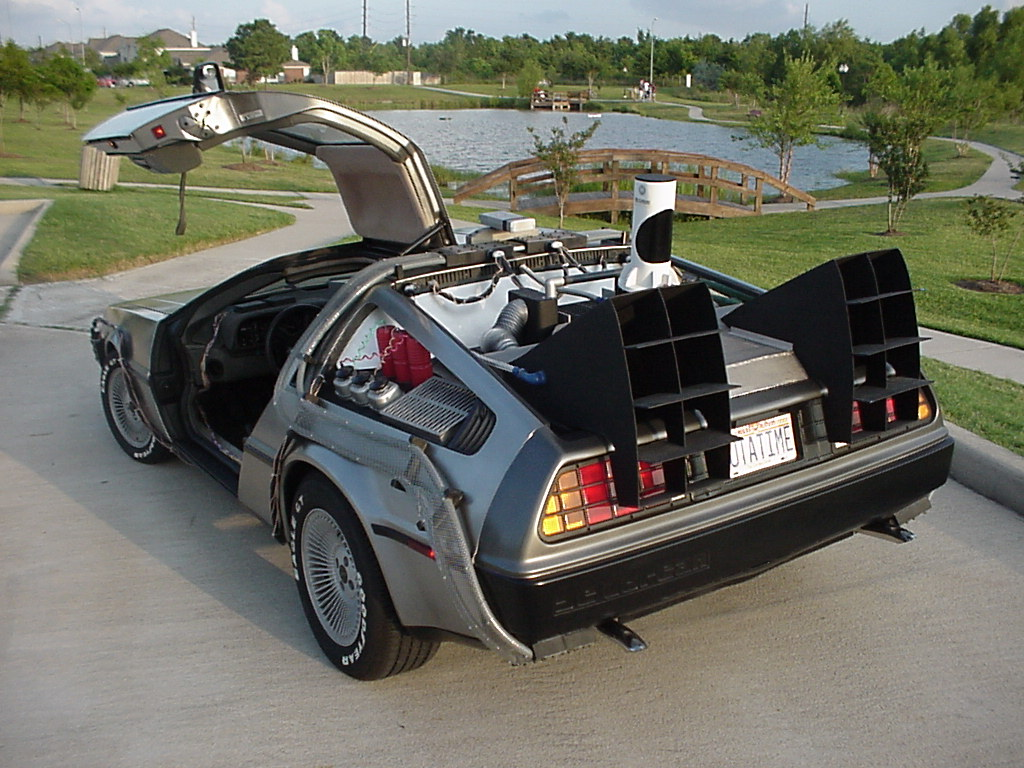
\includegraphics[width=0.45\textwidth]{./Figure/ExampleFigure1}
\caption{Esempio di figura.}
\label{FIG:Esempio di Figura}
\end{figure}

Esempio di tabella 
in tab.~\ref{TAB:Esempio}.

\begin{table}[htbp]
\centering
\begin{tabular}{ccc}
\toprule
Pilota 	& Giri 	& Sorpassi	\\
\midrule
Mario 	& 4/5 	& 5 				\\
Luigi 	& 3/5 	& 6 				\\
\bottomrule
\end{tabular}
\captionof{table}{Esempio con codice \LaTeX\ ordinato}
\label{TAB:Esempio}
\end{table}
Anche se non necessario, � meglio tenere la tabella ordinata... 
La tab.~\ref{TAB:Esempio} � uguale alla tab.~\ref{TAB:Esempio2}, ma osservando il listato \LaTeX\ la \ref{TAB:Esempio} � sicuramente pi� leggibile.
La cosa diventa utilissima per tabelle di grandi dimesioni.
\begin{table}[htbp]
\centering
\begin{tabular}{ccc}
\toprule
Pilota&Giri&Sorpassi\\
\midrule
Mario&4/5&5\\
Luigi&3/5&6\\
\bottomrule
\end{tabular}
\caption{Esempio con codice \LaTeX\ non ordinato}
%\captionof{table}{Esempio con codice \LaTeX\ non ordinato}
\label{TAB:Esempio2}
\end{table}

Notare l'inizio di un nuovo capoverso con questa frase\dots\
Ossevare il codice \LaTeX , � stata inserita una riga vuota dopo la tab.~\ref{TAB:Esempio2}. 
Tra la tab.~\ref{TAB:Esempio} e la tab.~\ref{TAB:Esempio2} invece no.